\section{交叉熵}
\label{sec:info-cross-entropy}

图~\ref{fig:info-question-tree}的提问方案是按真实概率$(\tfrac12,\tfrac14,\tfrac18,\tfrac18)$设计的：越常见的结果问得越少。如果设计者误以为四个字母等可能，就会给每个字母都安排两题；如果误以为概率是$(\tfrac18,\tfrac18,\tfrac14,\tfrac12)$，就会先问$d$、再问$c$，把最常见的$a$留到第三题。结果仍按真实分布出现，平均题数是多少，比按真实分布设计多出多少？

这类问题里有两个分布，角色不同。真实分布$P$决定结果出现的频率；参考分布$Q$决定给每个结果分配的代价$-\ln q(x)$，按$Q$看越常见的结果代价越小。平均代价按$P$计算。

\begin{definition}[交叉熵]
\label{def:info-cross-entropy}
设$P,Q$是可数集合$\mathcal{X}$上的概率分布，质量为$p,q$。$P$相对于参考分布$Q$的\term{交叉熵}（cross-entropy）是
\begin{equation}
  H(P,Q)=-\sum_{x\in\mathcal{X}}p(x)\ln q(x)=\mathbb{E}_{P}[-\ln q(X)]\in[0,+\infty],
  \label{eq:info-cross-entropy}
\end{equation}
约定$0\ln q=0$，而$p(x)>0$、$q(x)=0$的项为$+\infty$。若$P,Q$对同一参考测度（如Lebesgue测度）有密度$p,q$，在$\int p\lvert\ln q\rvert<\infty$时定义$H(P,Q)=-\int p\ln q$。
\end{definition}

$H(P,P)=H(P)$。离散时每一项$-p(x)\ln q(x)\geq0$，交叉熵总有意义。若真实分布给某个结果正概率，而参考分布给它零概率，这个结果的代价是无穷大，交叉熵也是无穷大：按参考分布设计的方案根本没有给它留位置。

\begin{theorem}[交叉熵的分解]
\label{thm:info-cross-entropy-decomposition}
设$P,Q$是可数集合上的概率分布，$H(P)<\infty$。则
\begin{equation}
  H(P,Q)=H(P)+D_{\mathrm{KL}}(P\Vert Q).
  \label{eq:info-cross-entropy-decomposition}
\end{equation}
所以$H(P,Q)\geq H(P)$，等号当且仅当$Q=P$。
\end{theorem}

\begin{proof}
若有$x$使$p(x)>0=q(x)$，则$P$不绝对连续于$Q$，两边都是$+\infty$。否则在$p(x)>0$的点，
\[
  -\ln q(x)=-\ln p(x)+\ln\frac{p(x)}{q(x)}.
\]
按$P$平均。第一项的期望是有限的$H(P)$，第二项的负部可积，期望是$D_{\mathrm{KL}}(P\Vert Q)\in[0,+\infty]$，所以期望可以拆开，得到式~\eqref{eq:info-cross-entropy-decomposition}。等号条件来自KL的零值条件。
\end{proof}

分解把平均代价分成两部分。$H(P)$是结果本身固有的不确定性，无论怎样设计都省不掉；$D_{\mathrm{KL}}(P\Vert Q)$是参考分布与真实分布不一致造成的额外代价。在所有参考分布中，交叉熵在$Q=P$时最小。若在一族参考分布中选使$H(P,Q)$最小的$Q$，由于$H(P)$不随$Q$改变，这等价于使$D_{\mathrm{KL}}(P\Vert Q)$最小；第~\ref{chap:distribution-approximation}章在一般分布族中研究这样的逼近。

\paragraph{四字母表的计算}
以bit为单位计算，此时$-\log_2q(x)$就是按$Q$设计的提问方案中$x$所需的题数。真实分布$P=(\tfrac12,\tfrac14,\tfrac18,\tfrac18)$，$H(P)=1.75$。取两个参考分布：
\[
  Q_1=(\tfrac14,\tfrac14,\tfrac14,\tfrac14),\qquad Q_2=(\tfrac18,\tfrac18,\tfrac14,\tfrac12).
\]
$Q_1$给每个字母$2$题，平均$2$题，所以$H(P,Q_1)=2$，$D_{\mathrm{KL}}(P\Vert Q_1)=0.25$。$Q_2$给$a,b,c,d$分别$3,3,2,1$题，平均
\[
  \tfrac12\cdot3+\tfrac14\cdot3+\tfrac18\cdot2+\tfrac18\cdot1=2.625,
\]
多付$0.875$题，这就是以bit计的$D_{\mathrm{KL}}(P\Vert Q_2)$。

\begin{BookInlineFigure}
  \centering
  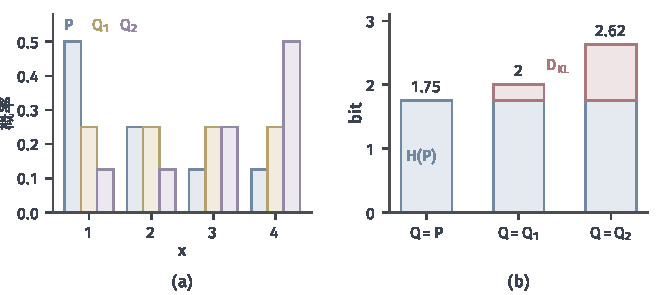
\includegraphics[width=112mm]{figures/07-probability/04-distribution-analysis/matplotlib/info-cross-entropy/figure.pdf}
  \caption{交叉熵的分解。(a)真实分布$P$（蓝）与两个参考分布$Q_1$（黄，均匀）、$Q_2$（紫）。(b)以bit计的$H(P,Q)$，蓝色部分是$H(P)=1.75$，红色部分是$D_{\mathrm{KL}}(P\Vert Q)$：$Q=P$时为$0$，$Q_1$时为$0.25$，$Q_2$时为$0.875$。}
  \label{fig:info-cross-entropy}
\end{BookInlineFigure}

图~\ref{fig:info-cross-entropy}显示，三种设计的蓝色部分一样高，差别全在红色部分。$Q_2$把最常见的结果当成最罕见的，失配最严重。

交叉熵的两个分布不能交换。真实分布为$Q_1$、参考分布为$P$时，四个字母等可能出现，而按$P$设计的题数是$1,2,3,3$，平均
\[
  H(Q_1,P)=\tfrac14(1+2+3+3)=2.25\neq H(P,Q_1)=2.
\]
两者的固有部分不同（$H(Q_1)=2$而$H(P)=1.75$），失配部分也不同（$0.25$与$0.25$恰好相等只是这个例子的巧合，一般不等）。若参考分布取$Q_3=(\tfrac12,\tfrac12,0,0)$，它完全没有为$c,d$留位置，$H(P,Q_3)=+\infty$。

\paragraph{熵为无穷时}
式~\eqref{eq:info-cross-entropy-decomposition}要求$H(P)<\infty$。若$H(P)=+\infty$，取$Q=P$，则$H(P,Q)=H(P)=+\infty$，而$D_{\mathrm{KL}}(P\Vert Q)=0$。这时“$D_{\mathrm{KL}}=H(P,Q)-H(P)$”是$\infty-\infty$，没有意义。KL散度直接由式~\eqref{eq:info-kl-recall}定义，不经过这个差。

\paragraph{连续情形}
对密度，交叉熵与微分熵一样依赖坐标。设$P=\mathcal{N}(0,1)$，$Q_s=\mathcal{N}(0,s^{2})$。参考分布分配的代价是
\[
  -\ln q_s(x)=\frac12\ln(2\pi s^{2})+\frac{x^{2}}{2s^{2}}.
\]
按$P$平均，用$\mathbb{E}_P[X^{2}]=1$，得到
\[
  H(P,Q_s)=\frac12\ln(2\pi s^{2})+\frac{1}{2s^{2}}.
\]
减去$h(P)=\tfrac12\ln(2\pi\mathrm{e})$，得到
\[
  D_{\mathrm{KL}}(P\Vert Q_s)=\ln s+\frac{1}{2s^{2}}-\frac12.
\]
$s=1$时为零；$s=2$时$H(P,Q_2)\approx1.737$，比$h(P)\approx1.419$多$0.318$。图~\ref{fig:info-gauss-cross}画出了整条曲线。

\begin{BookInlineFigure}
  \centering
  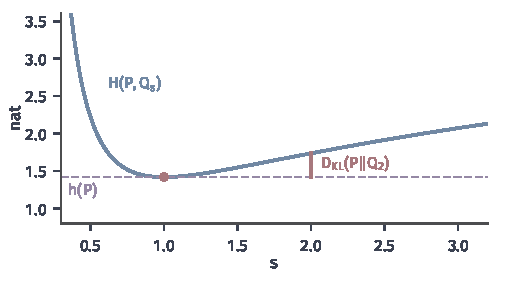
\includegraphics[width=86mm]{figures/07-probability/04-distribution-analysis/matplotlib/info-gauss-cross/figure.pdf}
  \caption{$P=\mathcal{N}(0,1)$相对于$Q_s=\mathcal{N}(0,s^{2})$的交叉熵（蓝），紫虚线为$h(P)\approx1.419$，单位nat。最小值在$s=1$（红点）处达到；红色竖线是$s=2$时的KL散度$0.318$。}
  \label{fig:info-gauss-cross}
\end{BookInlineFigure}

参考分布太窄（$s$小）时，交叉熵增长得很快：$P$的结果经常落在$Q_s$认为罕见的地方，每次都付很高的代价。太宽时增长较慢，只是对每个结果都略显“意外”。若把$x$换成$ax$，$h(P)$与$H(P,Q_s)$都增加$\ln\lvert a\rvert$，差$D_{\mathrm{KL}}$不变。连续情形下，有确定意义的是失配部分，而不是交叉熵本身的数值。

表~\ref{tab:info-entropy-cross}总结熵、交叉熵和KL散度的区别。

\begin{BookInlineTable}
  \centering
  \caption{熵、交叉熵与KL散度}
  \label{tab:info-entropy-cross}
  \begin{tabular}{@{}llll@{}}
    \toprule
    量 & 平均的对象 & 依赖坐标 & 下界\\
    \midrule
    $H(P)$或$h(P)$ & $P$下的$-\ln p$ & 连续时依赖 & 离散时$0$\\
    $H(P,Q)$ & $P$下的$-\ln q$ & 连续时依赖 & 离散时$H(P)$\\
    $D_{\mathrm{KL}}(P\Vert Q)$ & $P$下的$\ln(p/q)$ & 不依赖 & $0$\\
    \bottomrule
  \end{tabular}
\end{BookInlineTable}
